Dieser Versuchsteil befasst sich mit der grafischen Darstellung der Momentanleistung mithilfe eines Oszilloskopes. Der Verlauf von Strom und Spannung, deren Phasenverschiebung zueinander, und der Zusammenhang zum Verlauf der Momentanleistung wird betrachtet.


\subsubsection{Versuchsaufbau}

Abbildung \ref{fig:Plan2-1} zeigt den in diesem Versuchsteil verwendeten Schaltplan. Folgende Parameter werden verwendet:
\begin{itemize}
\item $Z_1 = \frac{1}{j\omega C} \mbox{ mit } C=4\mu F$
\item $Z_2 = 60\Omega$
\item $Z_3 = R_{sp} + j\omega L$ mit $R_{sp} = 5,5\Omega; L=15,84mH$
\item $u_{ges}$ wird durch Veränderung von $R_I$ auf 6V eingestellt.
\end{itemize}

\begin{figure}[h]
\centering
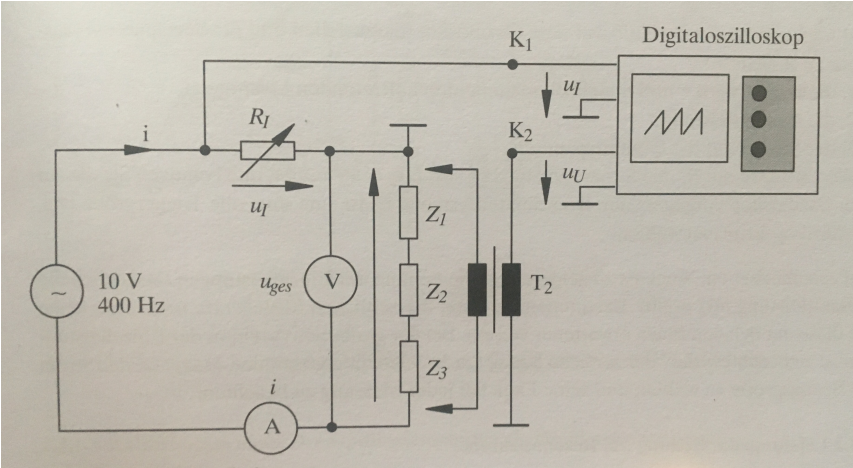
\includegraphics[width=0.7\linewidth]{Images/Aufbau2-1.png}
\caption{Schaltplan Versuch 2.1}
\label{fig:Plan2-1}
\end{figure}
\large{REFERENCE}

Im Folgenden wird das Oszilloskop zur Anzeige der Momentanleistung verwendet. Hierfür wird die Spannung über einen beliebigen Verbraucher mithilfe des potentialtrennenden Transformators $T_2$ am Oszilloskopeingang gemessen. Der Strom $i$ wird anhand der am Widerstand $R_I$ abfallenden Spannung gemessen. Zusätzlich lässt sich der Effektivwert des Stromes am Ampermeter ablesen.

Das Oszilloskop nun wird so eingestellt, dass das Produkt aus $u_I$ und $u_U$ angezeigt wird. Da $u_I$ proportional zu $i$ ist, wird so eine zur Momentanleistung proportionale Kurve angezeigt.

\subsection{Momentanleistungskurven}

Die im Folgenden dargestellten Kurven werden vom Oszilloskop abgespeichert. \textit{Ch~1} (blaue Kurve) stellt hierbei die zum Strom proportionale Kurve dar, \textit{Ch~2} (rote Kurve) die am Verbraucher gemessene Spannung. Die Momentanleistung $p(t)$ wird durch die grüne Kurve dargestellt.
\\
Folgende Kurven werden gemessen:

\paragraph{Momentanleistung am Kondensator}
Sie ist in Abbildung \ref{fig:MomLKurveZ1} dargestellt. Deutlich zu sehen ist die Phasenverschiebung von Strom und Spannung, welche bei ca. $\frac{\pi}{2}$ liegt. Die Kurve der Momentanleistung schwingt mit doppelter Frequenz um 0, besitzt also keinen Gleichanteil. Dies entspricht genau der Vorhersage von Gleichung \eqref{eq:MomLeistungSplit} bzw. \eqref{eq:LeistungGleichanteil}, welche für eine Phasenverschiebung von $\frac{\pi}{2}$ eine rein sinusförmige Schwingung und keine Wirkleistung vorhersagen. Der Kondensator nimmt somit entsprechend Gleichung \eqref{eq:KomplexS} eine Leistung von $\underline{S} = UIe^{-i\frac{\pi}{2}}$ auf.\par

\begin{figure}[H]
\centering
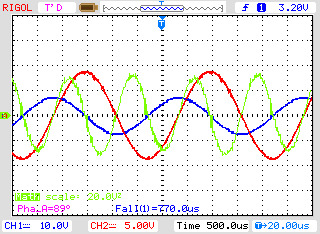
\includegraphics[width=0.6\linewidth]{Oszi-Bitmaps/NewFile0.jpg}
\caption{Momentanleistung am Kondensator. $u_I(t)$ (Blau), $u_{Z1}(t)$ (Rot), $p_{Z_1}(t)$ (Grün)}
\label{fig:MomLKurveZ1}
\end{figure}

\paragraph{Momentanleistung am Ohm'schen Widerstand}


\begin{figure}[H]
\centering
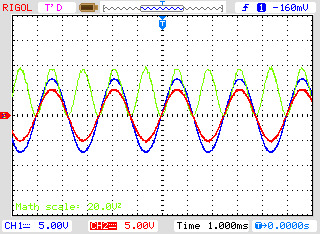
\includegraphics[width=0.6\linewidth]{Oszi-Bitmaps/NewFile1.jpg}
\caption{$p_{Z_2}(t)$}
\label{fig:MomLKurveZ2}
\end{figure}

\begin{figure}[H]
\centering
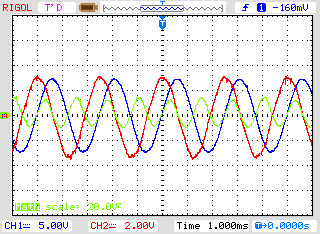
\includegraphics[width=0.6\linewidth]{Oszi-Bitmaps/NewFile2.jpg}
\caption{$p_{Z_3}(t)$}
\label{fig:MomLKurveZ3}
\end{figure}

\begin{figure}[H]
\centering
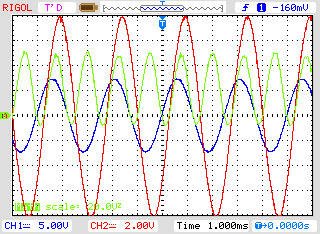
\includegraphics[width=0.6\linewidth]{Oszi-Bitmaps/NewFile3.jpg}
\caption{$p(t)$}
\label{fig:MomLKurveGesamt}
\end{figure}

Well Why not